\chapter{Concepts: Scala and DSLs}
\label{sec:concepts}

This part will first give a short overview of different features of Scala, followed by a basic
introduction to \dsls, tracing them into the history of programming languages and concluding with
the paradigm of language-oriented programming.


%%%%%%%%%%%%%%%%%%%%%%%%%%%%%%%%%%%%%%%%%%%%%%%%%%%%%%%%%%%%%%%%%%%%%%%%%%%%%%%%%%%%%%%%%%%%%%%%%%%%%
\section{Scala: Background and Paradigms}
\label{sec:scala}

Scala is a very flexible, multi-paradigm language, including a host of ideas by its
inventor Martin Odersky. For one, it provides advanced object-oriented constructs: almost everything
is in a class; there is a sophisticated type hierarchy; traits serve as \enquote{better interfaces},
and provide very flexible ways of inheritance, like mixins; there are a lot of constructs for
different aspects of class modelling, and they all can be nested. There is also a really smoothly
working and consistent module concept (which is probably influenced by Odersky's experience with
Modula-2). As a whole, Scala has been designed to serve as a multi-paradigm language, allowing
writing programs efficiently and expressively in the small as well as in the large scale~-- hence
also its name, stemming from \emph{scalable language}.

Furthermore, Scala is also quite a powerful statically typed functional language, not only providing
functions as first-order constructs with convenient syntax (as is minimally expected from a
functional language), but also being equipped with an elaborate type system, allowing to express
more things than in most other languages (like higher kinds, and certain types of
polymorphism). Also, the border to object-orientation is layed out in a very uncomplicated and
well-functioning way: case classes serve as class hierarchies as well as providing algebraic data
types (\abbrev{ADT}s), which can be pattern matched on, and the subtyping and parametric
polymorphism systems can be fused nicely by aid of type bounds and variance annotations.

Still, it is not only this wide semantic span of paradigms that makes Scala suited for a wide range
of use cases and architectorial considerations. There has been spent considerable amount of thought
on a lot of larger and smaller syntactic enhancements and shortcuts, most of which allow programmers
write code in a much more readable and natural way than usually. These features range from
\emph{string interpolation} and \emph{\abbrev{XML} literals} over \emph{blocks} and \emph{infix
  method calls} to quite unique inventions like \emph{implicit definitions}. The subsequent sections
will introduce the most useful of them for the development of \dsls, accompanied with examples of
their usage and patterns of combining them well.

\newthought{A few words on the level of details}: surely, one cannot explain a whole language
here. This text is also not an introduction to Scala. In general, it will always be tried to
explain as much as possible, using plenty of examples, so that a programmer having experience in a
few languages will be able to figure out what code means. However, some basic knowledge about Scala
syntax is assumed, as well as background knowledge about Java, functional programming, and some
aspects of semantics and type theory that are commonly discussed along with pure functional
programming. In particular, this concerns concepts related to types and functions, since functional
programming is considered a preliminary to all described aspects.

A more detailed foundation of Scala's syntactic features and standard libraries can be found in
Odersky's introductory book \citetitle{odersky2008:programming}~\cite{odersky2008:programming}, or
the Scala language specification~\cite{odersky2014:scala_spec}. Java, its \abbrev{API}, and the
\abbrev{JVM} are as well described in detail by their standardization
documents~\cite{gosling2013:java_spec, lindholm2013:jvm_spec, oracle:java_api_spec} (for
version~7). General introductions into common functional programming techniques are the
classic~\cite{abelson1996:structure} on the practical side (including untyped lambda calculus, pure
and impure functional programming and a general introduction into \dsl{} principles),
and~\cite{thompson1991:type}, going into theoretical foundations and type systems (especially higher
typed lambda calculi). A more thorough account of the practical type systematic approaches used in
Scala can be found in~\cite{pierce2002:types}, by which the language has noticably been influenced.

\newthought{The larger examples in this part} (listings on the top, marked with rules) are, in most
cases, published in a Github
repository\footnote{\protect\url{https://github.com/phipsgabler/dsl-examples}}, for the sake of
better reproducibility and further study. This repository containins a compileable \abbrev{SBT}
project with their implementations, and sometimes improvements, usage examples, and other
showcases. Such examples are marked and hyperlinked with an Octocat
icon~(\raisebox{-0.16em}{\github{dsl-examples}}).


%%%%%%%%%%%%%%%%%%%%%%%%%%%%%%%%%%%%%%%%%%%%%%%%%%%%%%%%%%%%%%%%%%%%%%%%%%%%%%%%%%%%%%%%%%%%%%%%%%%%%
\section{Overview: Why DSLs?}
\label{sec:overview}

Reviewing the history of computer science, as far as it is concerned with programming languages, one
can distinguish two great paradigms of how computation can be expressed (these are
\enquote{paradigms} more in an epistemiological than in a technical sense): \emph{imperative} and
\emph{declarative}. This distinction can be rooted in the earliest abstractions of computation that
were formulated, namely, Turing machines and the lambda calculus~\cite{valverde2015:punctuated}. As
has been early proved, both formulations are in fact equivalent; there is however a split, when
practically applying these concepts, which are purely mathematical at their core.

This split has its origins in the engineering perspective of programming, which strongly influenced
the evolution of programming languages. At the beginning of the usage of physical computers, all
there was was machine language, which was hand-written by specialized personnel (maybe using the
first assemblers, but not much more). Higher-level languages in these circles were believed to be a
purely academic exercise and not efficient enough in practice (not an unreasonable claim at the
time); it was not until the mid-fifties that they began being used. Then, between 1954 and 1957, the
ancestors of all modern imperative languages, Fortran, \abbrev{ALGOL}, and \abbrev{FLOW-MATIC} (soon
superseded by its more popular offspring \abbrev{COBOL}) were invented and became
popular~\cite{sammet1972:programming}.

What was convincing about these three languages was on the one hand the Fortran compiler's ability
to produce executables equivalently efficient to average hand-written machine language, but with
less effort of writing~-- this led to the general acceptance of compilation being feasible. On the
other hand, the idea behind \abbrev{FLOW-MATIC/COBOL} (and, to a lesser extend, \abbrev{ALGOL}) was
to allow programs to be written in English language, in a descriptive fashion completely unlike the
previously prevalent style of native instructions. Soon after this short phase, the number of
programming languages invented started to increase almost exponentially. Languages were designed for
different purposes and with different backgrounds: \abbrev{SQL} for relational algebra queries,
\abbrev{APL} for vectorized numerical computations, C for systems programming, and so on. What is
common to all languages in this tradition is their intertwined struggle between generality and
expressivity~-- some paths evolved to what is nowadays called \enquote{general-purpose} languages
(such as \CC), while others became more and more specialized and even lost their abilities for
programming in the whole (such as \abbrev{SQL}).

This language family has machine language as its proto-language, and its members are all based on
some form of compilation of a syntax to an underlying machine model, or, in the case of interpreted
languages, executing them step-by-step on such a model. They are thus, in a sense, Turing-oriented:
syntax is considered an extra layer above the actual execution on an abstract machine; and the
engineering perspective mentioned above came up because concrete computers are just instances of
such abstract machines.

There evolved however another language family, fundamentally different from this concept:
\abbrev{LISP} and its successors. In contrast to the languages mentioned above, \abbrev{LISP} had
never been designed as a successor to machine language. Instead, the initial idea was just a formal
lambda calculus with primitive types, macros, and better syntax (\enquote{recursive functions of
  symbolic expressions}); the actual implementation on a computer happened only \enquote{by
  accident}~\cite{mccarthy1960:recursive}. To this comes the fact that initially, the main user
group of the language was the \abbrev{AI} community, finding in it a way to concisely describe their
abstract concepts, regardless of underlying implementation.

While \abbrev{LISP} over the course of its growth incorporated also imperative parts, it is
fundamentally geared to the lambda calculus, with its term-rewriting style of thinking, reinforced
by its own homoiconicity. In this tradition, the language lead to the invention of techniques that
probably would not have been devised from the Turing perspective: these are, for example, the
first-class membership of functions and continuations, dynamic typing at runtime, and garbage
collection. Such concepts came into being because the language was used by people who were not using
it to write machine instructions on a higher level, but who approached programming from an almost
mathematical perspecitive, wanting to specify \emph{what} something shall be, not \emph{how} it
should be executed. In that way, \abbrev{LISP} pioneered the idea of considering programming
languages as an end in themselves.

\newthought{These are the historical foundations} of programming languages, summarized in
short. From them, we can learn how the means of expressing intent to a machine evolved, and from
what perspectives they started.

Nowadays, (most) people need not anymore be convinced that high-level languages are something
positive and worth while. The challenge is to overcome the view of code as something to be solely
compiled down, an intermediate, beneath form of thought, between the brain and the machine. If we
instead accept code as a form of language, and take its means of expression not as syntactic
niceties, but as fundamental properties of it as a system, new perspectives will come up. In that
spirit, Abelson and Sussman say in \citetitle{abelson1996:structure} that \blockcquote[][Preface to
the First Edition]{abelson1996:structure}[.]{(\ldots\kern-1pt) we want to establish the idea that a
  computer language is not just a way of getting a computer to perform operations but rather that it
  is a novel formal medium for expressing ideas about methodology. Thus, programs must be written for
  people to read, and only incidentally for machines to execute}
\setlength{\parskip}{0cm} % a hell of a hack because I don't know why \list{} is resetting
                          % \parskip in twopage output???

As we have seen above, programming languages tend to oscillate between extreme poles: imperative
versus declarative, and general versus specific. And as the complexity of systems and architectures
grows, and their construction becomes a more professional business, all these poles have proven
their value in some or the other way; but most importantly, it can be said that none of them is the
key to salvation on its own. In fact, successful complex systems most often rely on a patchwork of
multiple, specialized components, glued together by general frameworks of architecture. And if we
bend our concept names a bit, general-purpose languages could actually be considered special-purpose
for general \enquote{glue} code, and imperative code considered declarative descriptions of
imperative processes. 

If we so refrain from looking for \enquote{one language to rule them all}, and accept the above view
about the importance of languages in themselves, we arrive at a new point of view~-- in some form, a
new paradigm: \emph{language-oriented programming}~\cite{dmitriev2004:language}. Its philosopy is
exactly the just described manner of organizing systems: splitting them in smaller, coherent parts,
and program them out using the respective \emph{domain specific language}, which is a language as
close as possible to the terms and concepts of the specific part.

\newthought{This language-oriented paradigm} and its main constituents, \dsls{}, have actually been
around for some, often under different names, or in the context of other methodologies. For example,
the programming approach suggested in \cite{abelson1996:structure} is there called \emph{metalinguistic
  abstraction} and proposed as a rather general approach to problem solving; but then, there have
always been used small configuration or mini-languages for systems such \abbrev{UNIX} (like the
\texttt{sed} program), which are not backed by such a general idea, but just evolved as
practical. Moreover, there is range of highly specific languages to help with specialized tasks,
including the already mentioned \abbrev{SQL}, the grammar specification language of \abbrev{ANTLR}
or other parser generators, and \LaTeX. We can also regard special syntaxes for specific purposes as
a kind of \dsl{}, like Matlab's matrix literals and special operators, or the simulation statements
of hardware description languages such as Verilog.

A summary of the advantages of using \dsls{} is given in \cite{spinellis2001:notable}, which also
lists notable patterns found in the development process of them. \cite{mernik2005:dsls} offers an
overview of decision, analysis, design, and implementation phases of \dsl{} development, from a more
methodological view point, altough the work focuses more on external languages. Case studies for
\dsl{} development are~\cite{wile2004:lessons} with a lot of more abstract \enquote{lessons
  learned}, and~\cite{havelund2010:case}, which compares two implementations of the same \dsl{} in
Python and Scala with respect to their \enquote{linguistic elegance} (and even contrasts multiple
variations in Scala).

\label{dsl-definitions}
\newthought{With all this variety} of declarative and in some sense domain-specific languages, we
could try to classify them (see also \autoref{fig:dslterms}). The most prominent and used
distinction for \dsls{} is that between \emph{external} and \emph{internal} \dsls{}. Thereby, a
\dsl{} is called internal if it is used as part of another, more general programming language
(either through special syntax, or provided by a library), and called external, if it is executed by
a dedicated \enquote{evaluator} different from the main implementation language (which can be
anything from a compiler over an interpreter to a \abbrev{DBMS}).\footnote{Again, \abbrev{SICP}
  tries to be smarter than and blur this binary distinction:
  \textcquote[][Chapter~4]{abelson1996:structure}{The evaluator, which determines the meaning of
    expressions in a programming language, is just another program.}}

\begin{figure}
  \centering\sffamily
  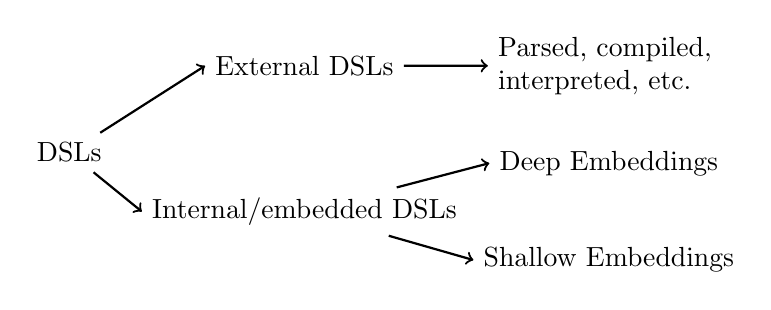
\begin{tikzpicture}[%
    ->, thick, grow=right,
    level 1/.style={level distance=8.5em},
    level 2/.style={level distance=11em, sibling distance=3.5em},
    child anchor=west]
    \node {DSLs}
    child {node [] {Internal/embedded DSLs}
      child {node {Shallow Embeddings}}
      child {node {Deep Embeddings}}}
    child {node [yshift=1em] {External DSLs}
      child {node [text width=8em] {Parsed, compiled, interpreted, etc.}}};
  \end{tikzpicture}
  \caption{Taxonomy of terms specifying the different variants of Domain Specific
    Languages.\label{fig:dslterms}}
\end{figure}

While external \dsls{} could arguably be differentiated in arbitrarily complex ways, some basic
further discrimination is practical for internal ones. For one, there are the two said possibilities
of having an internal \dsl{} provided by the language or via a library. The latter variant in the
following will be referred to as \emph{embedded}\footnote{As far as is known to the author, there is no
generally accepted convention for a clear distinction between the terms \enquote{embedded} and
\enquote{internal}, but this usage seems useful.}. It is embedded \dsls {} that this work focuses on,
since they are in a sense the most \enquote{language oriented}~-- using the features of a language
to extend itself.

Within the range of embedded \dsls{}, there is a further differentiation to be made: that of
\emph{deep} and \emph{shallow} embeddings. This distinction concerns the evaluation of the embedded
syntax: in a shallow embedding, the provided language constructs are merely combinators for some
already-existing objects in language, for example, they may simply be stacking functions in an
intricated way~-- but evaluation is not different from the normal language behaviour. In contrast, a
deep embedding uses an internal \abbrev{AST}, or at least some symbolic representation, together
with a custom evaluation function. The latter has the advantage that there is often more semantic
flexibility involved, and that there might be multiple evaluation functions provided
(\enquote{backends}); however, this usually comes with greater complexity and runtime or space
costs. A survey and comparison of both approaches can be found in~\cite{gibbons2014:folding}, which
uses a Haskell example.


%%% Local Variables: 
%%% TeX-master: "document"
%%% End: